\section{Design af user interfacet}
I dette afsnit vil vi beskrive det generelle design af brugergrænsefladen og de beslutninger der ligger bag.

\subsection{Et samlet overblik}
Da den første UI skulle designes hvade vi hele tiden i tankerne at den skulle være strømlignet og have et højt niveau af ease of use\footnote{User Interface Design, side 9}, vi havde derfor fokus på ikke at få lavet for mange skærmbilleder og sørge for at dem der var, var konsistense således at man højeste skulle kunne navigere rundt i to-tre af vinduerne for at man også ville kunne navigere rundt i resten.\\ Derudover ville vi også gerne have at UI'en virkede bekendt, vores udgangspunkt var derfor at prøve at lave et system som mindede om noget man var vant  til at se fra andre booking systemer.
Da vi gik efter at have et højt niveau af ease of use ville vi derfor gerne lave programmet til en platform som var nem at arbejde med og nemt tilgængelig, vi valgte derfor at lave GUI'en som en website  da det ville gøre den nemmere tilgængelig for flere og igen sørge for at det ville være nemt og hurtigt at bruge systemet.

\subsection{Booking metoden}
Som nævnt ville vi gerne prøve at efterligne eksisterende booking systemer, specielt blev vi meget inspireret af biografbooking dette skyldes at det er et meget intuitivt systmet hvilket vi gerne også vil opnå.\\ Konceptet med at visuelt vælge hvad man vil have og deres simple farvekodning var noget der passede godt ind i vores koncept med ease of use og intuitivt design.
\begin{figure}[h!]
  \caption{screenshot af kino.dk's booking interface.}
  \centering
    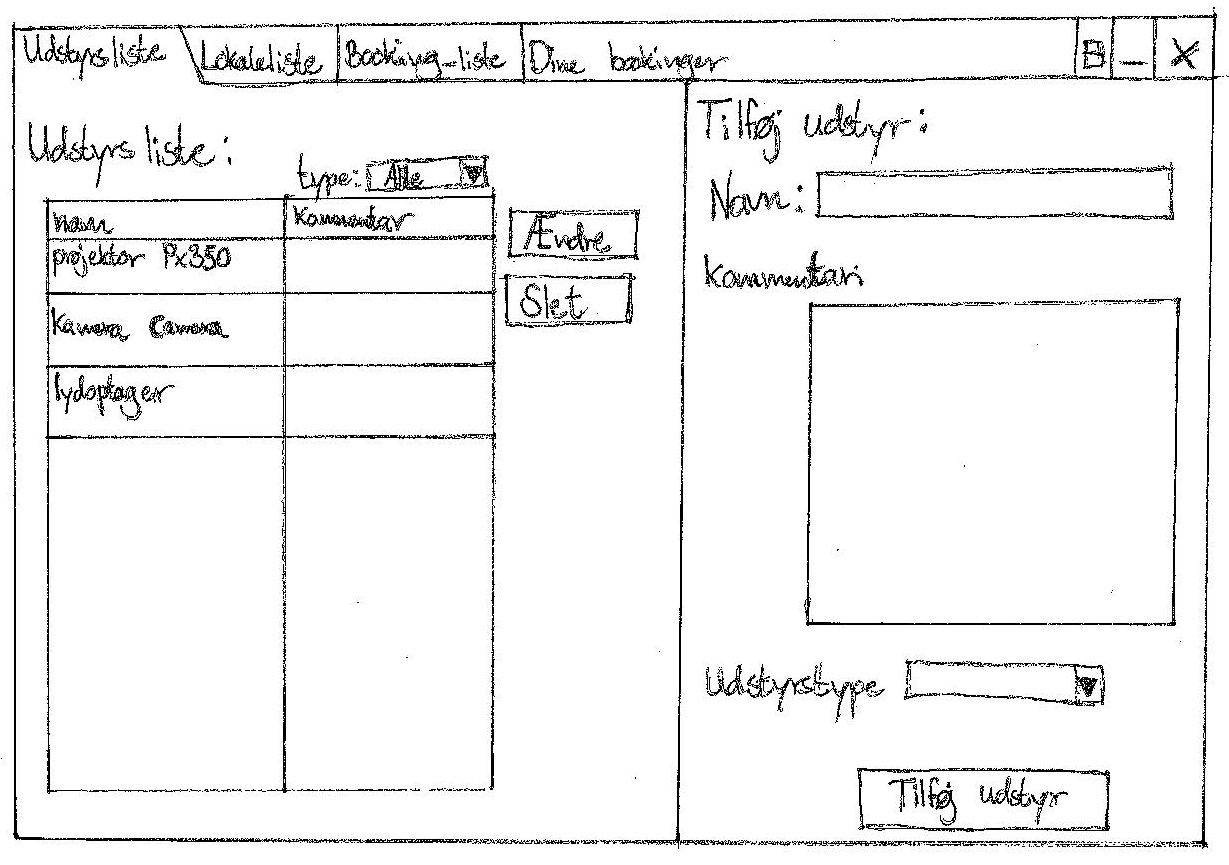
\includegraphics[width=0.5\textwidth]{Appendix/GUI-Prototype/PaperMockup/UdstyrsListe}
\end{figure}


Vi valgte derfor at prøve at efterligne det ved at lave et gitter hvor man kunne klikke i felterne for at booke et lokale i det tilsvarende tidsrum, det viste sig dog af vores første usability test\footnote{resultat af usability test1}, at den løsning ikke var helt brugervenlig nok vi valgte derfor at tilføje checkboxses til alle felterne for at gøre det mere tydeligt at det var det der skulle markes for at booke i et givent tidsrum.
\begin{figure}[h!]
  \caption{Den endelige udgave af gitter skærmbilleder til booking.}
  \centering
    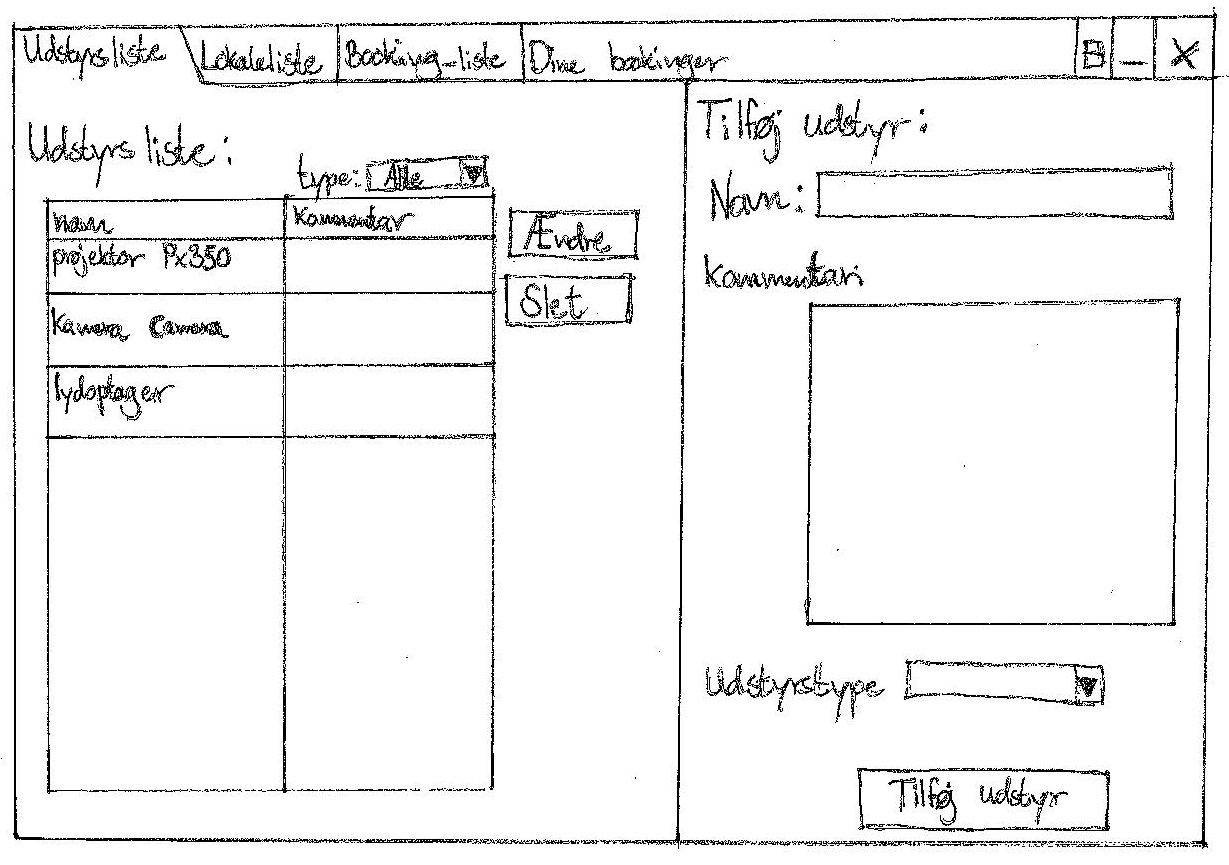
\includegraphics[width=0.5\textwidth]{Appendix/GUI-Prototype/PaperMockup/UdstyrsListe}
\end{figure}
\\Da vi gerne vil opnå en brugergrænseflade som var strømlignet og nem at bruge, brugte vi også gitter løsningen til alt andet der relaterede til en booking i systemt såsom tilføjelse af  udstyr og forplejning. Til resten af skærm billederne har vi holdt os til simple billeder der fokusere på kun at præsentere dataen og de nødvendige knapper.

\subsection{UI'ens udvikling og udseende}
Til UI'ens generelle udseende gik vi efter at der skulle være meget få forskellige skærmbilleder således at der måske var 10-15 skærmbilleder, men for brugen skulle vedkommende kun lære at navigere igennem et par stykker for at kunne navigere igennem resten.
Generelt kan man opdele vores skærmbilleder i to typer, den første type var dem som alle indholdte booking gitterer i og med de alle vil fungere på samme måde med at man checker i de checkboxses man gerne ville booke og så godkende bookingen.
Ovenfor er et screenshot af vores endelig design af et gitter skærmbillederne.
\begin{figure}[h!]
  \caption{første udgave af gitter skærmbilleder til booking.}
  \centering
    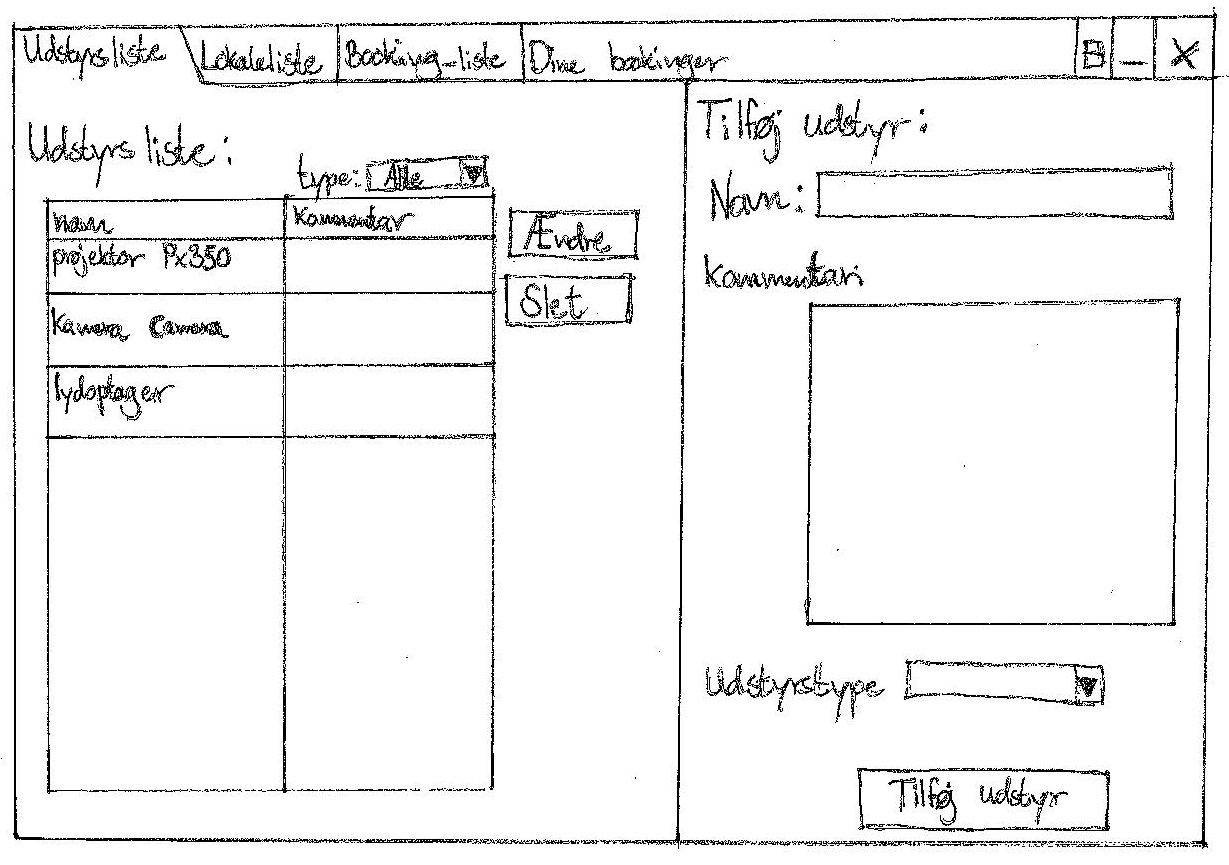
\includegraphics[width=0.5\textwidth]{Appendix/GUI-Prototype/PaperMockup/UdstyrsListe}
\end{figure}


Ovenfor er vist det skærmbilled der blev brugt til at lave den første runde af usability test på en simpel papirmockup, som man kan se minder den i sin form om det endelig version men der nogle små forskelle, det vigtigste er tilføjelsen af checkboxses. Disse blev tilføjet efter første runde af usabilitytests da feedbacken var at der mangler noget man kunne klikke på i gitteret, derudover gjorde vi også knapperne mere merkante og gav dem i fælles layout så det var meget tydligt hvad der var klikbare knapper.

Den anden type af skærmbilleder er primært til editering i de forskellige tabeller der er i systemet det kunne eksempelvis være oversigten over lokaler hvor man er i stand til at ændre, slette og tilføje lokaler.
I den første udgave i papir mockupen var disse meget simple og manglede noget information om hvad der blev vist.
\begin{figure}[h!]
  \caption{første udgave af skærmbilled over en liste af bookinger der skal godkendes af receptionisten.}
  \centering
    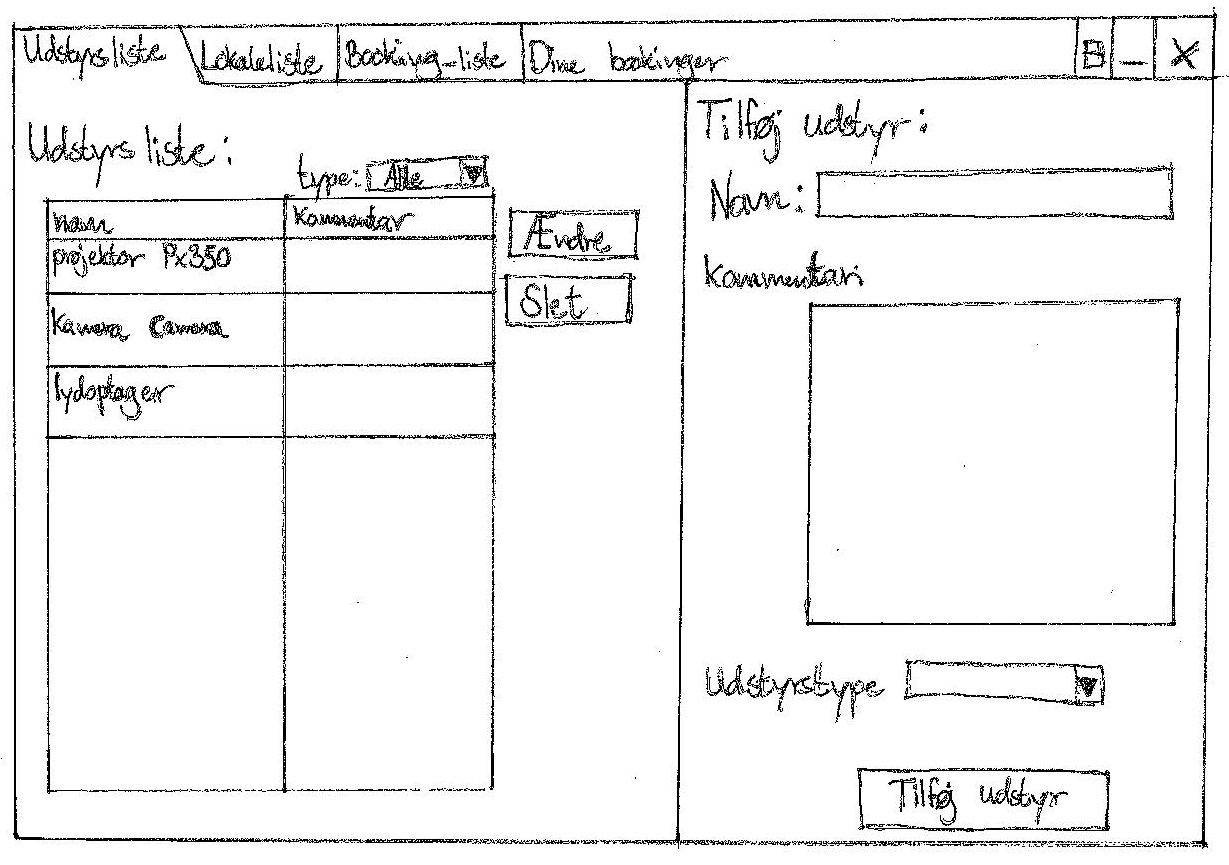
\includegraphics[width=0.5\textwidth]{Appendix/GUI-Prototype/PaperMockup/UdstyrsListe}
\end{figure} 
I forhold til det generelle design af skærmbillederne prøvede vi at gøre dem simple og at overholde gestalt lovene\footnote{User Interface Design, side 68} specifikt Law of proximity. Således at det virker som om knapper intuitivt tilhører til den liste, som de interegere med.




